\section{Theory}
\label{sec:theory}

This section states what can be proved about the band and what can only be conjectured, with the conditions under which each
statement holds. Throughout, the marginals satisfy the standing assumption of Section~\ref{sec:problem-assumptions}: each $Q_k$ is
continuous and strictly increasing on the region where it is read. The results are labelled [D] when they are derived here or
quoted from the cited source with its proof, and [C] when they are conjectures supported by the experiments.

\subsection{The headline is the comonotonic capital, and the expected shortfall bounds every row}
\label{sec:theory-headline}

\begin{proposition}[Headline and ceiling] [D]
\label{prop:headline}
Let $\pi_{\mathrm{com}}$ be the comonotonic coupling, the law of $(Q_1(U),\dots,Q_K(U))$ for one uniform variable $U$. Then
\begin{equation}
b(\pi_{\mathrm{com}})=H=\sum_k\mathrm{EC}_k .
\label{eq:comonotonic}
\end{equation}
For every coupling $\pi\in\mathcal C$,
\begin{equation}
b(\pi)\le\sum_{k=1}^K\ES_\alpha(L_k)-\sum_{k=1}^K\mathrm{EL}_k ,
\label{eq:es-ceiling}
\end{equation}
and the value at risk of the total can exceed $\sum_k\VaR_\alpha(L_k)$, so that $\overline b>H$ is possible.
\end{proposition}

\begin{proof}
Under $\pi_{\mathrm{com}}$ the total is $S=g(U)$ with $g=\sum_kQ_k$, which is continuous and strictly increasing by the standing
assumption. Then $\Prob(S\le x)=g^{-1}(x)$ on the range of $g$, so $\VaR_\alpha(S)=g(\alpha)=\sum_kQ_k(\alpha)=\sum_k\VaR_\alpha(L_k)$.
Subtracting $\sum_k\mathrm{EL}_k$ gives Equation~\ref{eq:comonotonic}. For Equation~\ref{eq:es-ceiling}, the expected shortfall
is the mean of the quantiles above $\alpha$, each at least $Q_S(\alpha)$, so $\VaR_\alpha(S_\pi)\le\ES_\alpha(S_\pi)$; the expected
shortfall is subadditive \citep{acerbi2002,artzner1999}, so $\ES_\alpha(S_\pi)\le\sum_k\ES_\alpha(L_k)$. The last claim is not a
consequence of the first two: the value at risk is not subadditive, and the sharp worst case of Section~\ref{sec:results-band} is
an instance with $\overline b>H$ \citep{ems2002,epr2013}.
\end{proof}

The proposition says two things about the band. The simple sum is not an arbitrary figure: it is the capital of the one coupling
in which the risk types reach their quantiles together. And the simple sum is not a ceiling either, since a coupling that is not
comonotonic can put more of the loss above the quantile. The ceiling that does hold is the sum of the expected shortfalls, which
for Banco Andino is CLP \bdSumEs{} billion of value at risk against the worst case of CLP \bdWorstVar{} billion, a slack of
CLP \bdSlack{} billion that the numerical bound must respect (Section~\ref{sec:results-structure}).

\subsection{Bracketing and invariance of the bounds}
\label{sec:theory-bracket}

\begin{proposition}[Bracket and invariance] [D]
\label{prop:bracket}
For every coupling $\pi\in\mathcal C$, $\underline b\le b(\pi)\le\overline b$. In particular every row of the band that is the
capital of a coupling lies in $[\underline b,\overline b]$: the simple sum, the Gaussian copula row and each $t$ copula row. The
numbers $\underline b$ and $\overline b$ are functions of $(Q_1,\dots,Q_K,\alpha)$ and of $\sum_k\mathrm{EL}_k$ only, so they do
not change with the correlation matrix, with the degrees of freedom or with any other dependence input.
\end{proposition}

\begin{proof}
The first claim is the definition of the infimum and the supremum in Equation~\ref{eq:sharp-bounds}. The rows named are capitals of
couplings: $\pi_{\mathrm{com}}$ by Proposition~\ref{prop:headline}, and the Gaussian and $t$ copulas with the marginals $Q_k$ by
Equation~\ref{eq:copula-sampling}. The set $\mathcal C$ and the functional $\VaR_\alpha(S_\pi)$ are defined from the marginals and
the level alone, so the bounds cannot depend on $R$ or $\nu$.
\end{proof}

Two limits belong to the statement. The square-root row of Equation~\ref{eq:sqrt-row} is not in general the capital of a coupling,
so Proposition~\ref{prop:bracket} does not place it in the interval, and the bracket test exists to check that it falls inside.
And the rearrangement algorithm that computes the bounds has no proof of convergence for all initial configurations: its authors
state a proof of convergence as an open problem \citep{puccetti2012,hofert2015}. The evidence that the algorithm has converged on
the marginals of the study is empirical: four independent runs end in ranges whose widths are
CLP \bdLowerRangeWidth{} billion for the lower bound and CLP \bdUpperRangeWidth{} million for the worst case
(Section~\ref{sec:results-structure}). Figure~\ref{fig:rearrangement} shows what the algorithm does to the tail of the study.

\begin{figure}[htbp]
\centering
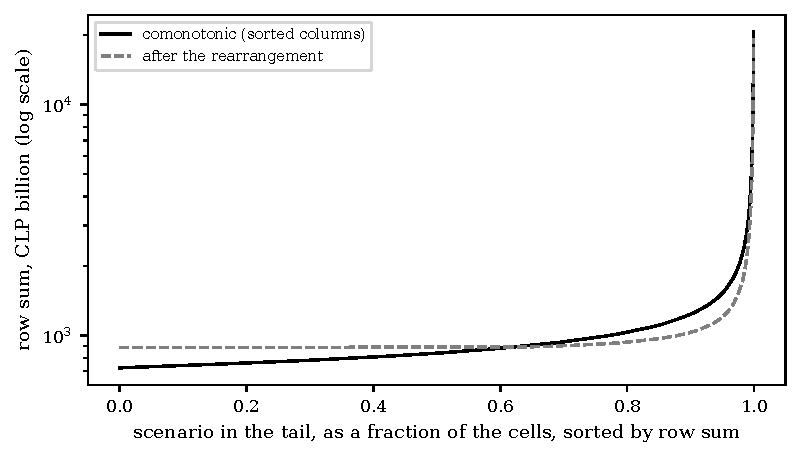
\includegraphics[width=0.78\textwidth]{figures/rearrangement}
\caption{The row sums of the $\bdRearrCells$ upper-tail cells of the four marginals of Banco Andino, in CLP billion on a logarithmic scale and sorted: with the columns sorted alike (comonotonic, solid line) and after the rearrangement of each column against the sum of the others (dash-dotted line). The smallest row sum rises from CLP \bdRearrMinComo{} to \bdRearrMinAfter{} billion, the worst value at risk, because the large losses of one risk type are moved to the cells where the others are small.}
\label{fig:rearrangement}
\end{figure}

\subsection{Dependence that the matrix does not carry}
\label{sec:theory-tails}

\begin{proposition}[Same rank correlation, different tails] [D]
\label{prop:tails}
Let $C^{\mathrm G}_R$ and $C^{t}_{R,\nu}$ be the Gaussian copula and the $t$ copula with the same correlation matrix $R$. Kendall's
rank correlation of the pair $(i,j)$ is the same for both,
\begin{equation}
\tau_{ij}=\frac{2}{\pi}\arcsin\rho_{ij},
\label{eq:kendall}
\end{equation}
and their upper tail dependence coefficients differ: for $\lvert\rho\rvert<1$ the Gaussian coefficient is zero, while the $t$
coefficient is
\begin{equation}
\lambda_\nu(\rho)=2\,t_{\nu+1}\!\left(-\sqrt{\frac{(\nu+1)(1-\rho)}{1+\rho}}\right)>0 ,
\label{eq:tail-dependence}
\end{equation}
which tends to zero as $\nu\to\infty$.
\end{proposition}

\begin{proof}
Equation~\ref{eq:kendall} holds for every elliptical distribution with continuous margins \citep{lindskog2003}. The tail
dependence coefficients of the Gaussian and the $t$ copulas are derived in \citet{demarta2005} and \citet{ems2002}: the
Gaussian coefficient vanishes for $\rho<1$ because the conditional law of one standardised variable given a large value of the
other is centred at $\rho$ times that value, and the $t$ coefficient follows from the same conditioning with the
$t_{\nu+1}$ law of the standardised residual. As $\nu\to\infty$ the argument of $t_{\nu+1}$ in Equation~\ref{eq:tail-dependence}
tends to $-\infty$ at the rate $\sqrt\nu$ and the coefficient to zero.
\end{proof}

At the pair correlation $\rho=0.5$ of the base matrix the coefficient is $\bdTLambdaFour$ for $\nu=4$ and $\bdTLambdaThirty$ for
$\nu=30$, and at $\rho=0.2$ it is $\bdTLambdaLowFour$ for $\nu=4$. The consequence for the band is that the three $t$ rows and
the Gaussian row share one matrix and one rank correlation and differ only in the tail dependence at the level where the capital
is read. That is why a correlation matrix alone cannot report the dependence uncertainty of the aggregate, and why the band holds
several degrees of freedom and not one.

\begin{remark}[Monotone in the degrees of freedom] [C]
\label{conj:nu}
For positively correlated risks with the marginals of the study, the capital of the $t$ copula row decreases as $\nu$ increases
and approaches the Gaussian row. The mechanism is the decrease of $\lambda_\nu(\rho)$ with $\nu$. The evidence is the curve of
Figure~\ref{fig:nu-curve} for the base and for the stressed matrix over eight values from 2.5 to 100: the capital is non-increasing
in $\nu$ up to two combined standard errors on both matrices, and at $\nu=100$ it exceeds the Gaussian row by CLP \bdNuHundredGap{}
billion, within the Monte Carlo error. It is a conjecture because the dependence of a quantile of a sum on $\nu$ can be non-monotone
for marginals with another shape of tail, and no proof is offered for the marginals of the study.
\end{remark}

\subsection{Closed forms for the square-root row and the allocation}
\label{sec:theory-closed}

\begin{proposition}[Shift of the square-root row] [D]
\label{prop:sqrt}
Let $\mathrm{EC}\ge0$ and let $R'$ differ from $R$ only in the pair $(i,j)$, where $\rho_{ij}'=\rho_{ij}+\Delta$. Then
\begin{equation}
b_{\mathrm{sqrt}}(R')^2-b_{\mathrm{sqrt}}(R)^2=2\Delta\,\mathrm{EC}_i\,\mathrm{EC}_j .
\label{eq:sqrt-shift}
\end{equation}
If every entry of $R$ lies in $[0,1]$, then $\sqrt{\sum_k\mathrm{EC}_k^2}\le b_{\mathrm{sqrt}}\le H$.
\end{proposition}

\begin{proof}
Write $\mathrm{EC}^\top R\,\mathrm{EC}=\sum_k\mathrm{EC}_k^2+2\sum_{k<l}\rho_{kl}\mathrm{EC}_k\mathrm{EC}_l$ and take the difference
for the two matrices, in which only the term $(i,j)$ changes. For the bounds, replace every off-diagonal entry by 0 for the lower
bound and by 1 for the upper bound, using $\mathrm{EC}\ge0$; the upper bound is $\sqrt{(\sum_k\mathrm{EC}_k)^2}=H$.
\end{proof}

For Banco Andino the stress that raises the market-credit correlation from 0.5 to 0.8 gives, by Equation~\ref{eq:sqrt-shift},
a change of $2\cdot0.3\cdot\mathrm{EC}_{\mathrm{credit}}\mathrm{EC}_{\mathrm{market}}=\bdVcClosedDiff\times10^{9}$ in CLP million
squared, and the committed rows give $\bdVcSquareDiff\times10^{9}$: the identity is met by the committed documents to the digits
shown. The floor of the proposition is CLP \bdSqrtFloor{} billion and the ceiling is the headline of CLP \bdHeadline{} billion;
the square-root row of CLP \bdVc{} billion lies between them.

\begin{proposition}[Additivity of the allocation] [D]
\label{prop:euler}
With the weights of Equation~\ref{eq:euler}, $\sum_kc_k=\widehat{\ES}_\alpha$ for every sample. If $\ES_\alpha$ is
differentiable in the weights, the contribution $c_k$ is its derivative with respect to the weight of risk type $k$ at the unit
weights.
\end{proposition}

\begin{proof}
For each draw $\sum_kL_{ik}=S_i$, so $\sum_kc_k=(1-\alpha)^{-1}\sum_iw_iS_i=\widehat{\ES}_\alpha$. The expected shortfall of
$\sum_kw_kL_k$ is positively homogeneous of degree one in $w$, so Euler's theorem on homogeneous functions gives
$\sum_kw_k\,\partial\ES_\alpha/\partial w_k=\ES_\alpha$; the identification of the derivative with the conditional expectation of
$L_k$ given the tail event is the Euler principle \citep{tasche2008}.
\end{proof}

The additivity is therefore an identity of the estimator, and a test of it checks the implementation. What is not an identity
is the allocation itself, which carries the sampling error of the tail of the sample: the shares in Table~\ref{tab:euler} have a
standard deviation of about one percentage point over independent seeds.

\subsection{Sampling error, and what coverage by the sharp range means}
\label{sec:theory-sampling}

The simulated rows are sample quantiles at $\alpha=0.999$, which rest on the $n(1-\alpha)$ largest draws, 1,000 of the $10^6$.
For independent draws the standard error of the sample quantile of the total is, asymptotically,
\begin{equation}
\mathrm{se}(\widehat q_\alpha)\approx\frac{\sqrt{\alpha(1-\alpha)/n}}{f_S(q_\alpha)} ,
\label{eq:quantile-se}
\end{equation}
with $f_S$ the density of the total \citep{glasserman2003}; the engine estimates it by batch means, without the density. The
error is below one percent of a row ($\bdGaussSd$ CLP billion on the Gaussian row over independent seeds)
and it is two orders of magnitude below the width of the band, which is the reason the rows can be compared (Section~\ref{sec:results-band}).

\begin{proposition}[Coverage by the sharp range] [D]
\label{prop:coverage}
Let $\pi^\ast\in\mathcal C$ be any planted dependence structure with the marginals $Q_k$. Then $b(\pi^\ast)\in[\underline b,\overline b]$.
\end{proposition}

\begin{proof}
It is the first claim of Proposition~\ref{prop:bracket} applied to $\pi^\ast$.
\end{proof}

The proposition has a consequence for the design. The coverage of the planted structures by the sharp range cannot be an
empirical finding about the structures: it holds for every structure, up to the error of the three estimated quantities, the
capital of the structure and the two ends of the range. The experiment that measures it is a verification of the implementation
against the theory, and its empirical content is the width of the interval, that is, how much of the interval is slack for the
structures that a bank might plausibly face. The interior rows are different. The interval spanned by the five interior rows is the
range of the capitals of five specific couplings, and whether it contains the capital of another coupling is an empirical question
that depends on the coupling: Proposition~\ref{prop:tails} says that a structure whose tail dependence or whose matrix lies outside
what the five rows span can fall outside. Section~\ref{sec:results-planted} measures it.
